%% For double-blind review submission, w/o CCS and ACM Reference (max submission space)
%\documentclass[sigplan,review,anonymous]{acmart}\settopmatter{printfolios=true,printccs=false,printacmref=false}
%% For double-blind review submission, w/ CCS and ACM Reference
%\documentclass[sigplan,review,anonymous]{acmart}\settopmatter{printfolios=true}
%% For single-blind review submission, w/o CCS and ACM Reference (max submission space)
%\documentclass[sigplan,review]{acmart}\settopmatter{printfolios=true,printccs=false,printacmref=false}
%% For single-blind review submission, w/ CCS and ACM Reference
%\documentclass[sigplan,review]{acmart}\settopmatter{printfolios=true}
%% For final camera-ready submission, w/ required CCS and ACM Reference
%\documentclass[sigplan]{acmart}\settopmatter{}

\documentclass[sigplan]{acmart}\settopmatter{printccs=false,printacmref=false}

%% Conference information
%% Supplied to authors by publisher for camera-ready submission;
%% use defaults for review submission.
\acmConference[PL'18]{ACM SIGPLAN Conference on Programming Languages}{January 01--03, 2018}{New York, NY, USA}
\acmYear{2018}
\acmISBN{} % \acmISBN{978-x-xxxx-xxxx-x/YY/MM}
\acmDOI{} % \acmDOI{10.1145/nnnnnnn.nnnnnnn}
\startPage{1}

%% Copyright information
%% Supplied to authors (based on authors' rights management selection;
%% see authors.acm.org) by publisher for camera-ready submission;
%% use 'none' for review submission.
\setcopyright{none}
%\setcopyright{acmcopyright}
%\setcopyright{acmlicensed}
%\setcopyright{rightsretained}
%\copyrightyear{2018}           %% If different from \acmYear

%% Bibliography style
\bibliographystyle{ACM-Reference-Format}
%% Citation style
%\citestyle{acmauthoryear}  %% For author/year citations
%\citestyle{acmnumeric}     %% For numeric citations
%\setcitestyle{nosort}      %% With 'acmnumeric', to disable automatic
                            %% sorting of references within a single citation;
                            %% e.g., \cite{Smith99,Carpenter05,Baker12}
                            %% rendered as [14,5,2] rather than [2,5,14].
%\setcitesyle{nocompress}   %% With 'acmnumeric', to disable automatic
                            %% compression of sequential references within a
                            %% single citation;
                            %% e.g., \cite{Baker12,Baker14,Baker16}
                            %% rendered as [2,3,4] rather than [2-4].


%%%%%%%%%%%%%%%%%%%%%%%%%%%%%%%%%%%%%%%%%%%%%%%%%%%%%%%%%%%%%%%%%%%%%%
%% Note: Authors migrating a paper from traditional SIGPLAN
%% proceedings format to PACMPL format must update the
%% '\documentclass' and topmatter commands above; see
%% 'acmart-pacmpl-template.tex'.
%%%%%%%%%%%%%%%%%%%%%%%%%%%%%%%%%%%%%%%%%%%%%%%%%%%%%%%%%%%%%%%%%%%%%%


%% Some recommended packages.
\usepackage{booktabs}   %% For formal tables:
                        %% http://ctan.org/pkg/booktabs
\usepackage{subcaption} %% For complex figures with subfigures/subcaptions
                        %% http://ctan.org/pkg/subcaption

\usepackage{calc}
\usepackage{enumitem}
\usepackage{stmaryrd}
\usepackage{tikz}
\usepackage{wrapfig}

\usetikzlibrary{calc}
\usetikzlibrary{decorations.pathreplacing}


\begin{document}

%% Title information
\title{DSLs for Protocols: Open Problems}         %% [Short Title] is optional;
                                        %% when present, will be used in
                                        %% header instead of Full Title.
%\titlenote{with title note}             %% \titlenote is optional;
                                        %% can be repeated if necessary;
                                        %% contents suppressed with 'anonymous'
%\subtitle{subtitle}                     %% \subtitle is optional
%\subtitlenote{with subtitle note}       %% \subtitlenote is optional;
                                        %% can be repeated if necessary;
                                        %% contents suppressed with 'anonymous'


%% Author information
%% Contents and number of authors suppressed with 'anonymous'.
%% Each author should be introduced by \author, followed by
%% \authornote (optional), \orcid (optional), \affiliation, and
%% \email.
%% An author may have multiple affiliations and/or emails; repeat the
%% appropriate command.
%% Many elements are not rendered, but should be provided for metadata
%% extraction tools.

%% Author with single affiliation.
\author{Sung-Shik Jongmans}
%\authornote{with author1 note}          %% \authornote is optional;
                                        %% can be repeated if necessary
%\orcid{nnnn-nnnn-nnnn-nnnn}             %% \orcid is optional
\affiliation{
%  \position{Position1}
  \department{Department of Computer Science}              %% \department is recommended
  \institution{Open University of the Netherlands}            %% \institution is required
%  \streetaddress{Street1 Address1}
%  \city{City1}
%  \state{State1}
%  \postcode{Post-Code1}
%  \country{Country1}                    %% \country is recommended
}
\email{ssj@ou.nl}          %% \email is recommended


%% Abstract
%% Note: \begin{abstract}...\end{abstract} environment must come
%% before \maketitle command
%\begin{abstract}
%Text of abstract \ldots.
%\end{abstract}


%%% 2012 ACM Computing Classification System (CSS) concepts
%%% Generate at 'http://dl.acm.org/ccs/ccs.cfm'.
%\begin{CCSXML}
%<ccs2012>
%<concept>
%<concept_id>10011007.10011006.10011008</concept_id>
%<concept_desc>Software and its engineering~General programming languages</concept_desc>
%<concept_significance>500</concept_significance>
%</concept>
%<concept>
%<concept_id>10003456.10003457.10003521.10003525</concept_id>
%<concept_desc>Social and professional topics~History of programming languages</concept_desc>
%<concept_significance>300</concept_significance>
%</concept>
%</ccs2012>
%\end{CCSXML}
%
%\ccsdesc[500]{Software and its engineering~General programming languages}
%\ccsdesc[300]{Social and professional topics~History of programming languages}
%%% End of generated code


%% Keywords
%% comma separated list
%\keywords{keyword1, keyword2, keyword3}  %% \keywords are mandatory in final camera-ready submission


%% \maketitle
%% Note: \maketitle command must come after title commands, author
%% commands, abstract environment, Computing Classification System
%% environment and commands, and keywords command.
\maketitle
\raggedbottom

\newcommand{\code}[2][\small]{{#1\texttt{#2}}}

\section{Introduction}

With the advent of multicore processors, concurrent programming has become an
important skill for many to acquire. However, concurrent programming remains
difficult: despite contemporary general-purpose languages (GPL) offering
higher-level abstractions on top of bare threads and locks, %(e.g., the
% fork/join framework in Java; actors in Scala and Erlang;
%channel-based message-passing in Go and Rust),
developers continue to struggle with classical concurrency errors, such as
deadlocks and data races~\cite{DBLP:journals/jisa/AsadollahSEH17}.

A major challenge that developers of concurrent programs face, pertains to the
implementation of \emph{protocols} (i.e., synchronization\slash communication
patterns) among \emph{tasks} (i.e., sequential computations, run concurrently):
although GPLs offer concurrency primitives to implicitly enact global
\emph{interactions} of protocols (e.g., a communication of an integer from task
$T_1$ to $T_2$) indirectly through local \emph{actions} of tasks (e.g., $T_1$
writes integer \code{5} to variable \code{x}, then releases to semaphore
\code{s}; concurrently, $T_2$ blocks until it acquires from \code{s}, then reads
from \code{x}), GPLs lack linguistic support to explicitly enact interactions,
directly. Aggravated by the exponentially many, seemingly nondeterministic,
interleavings in which tasks can be scheduled, purely \emph{action-centric
protocol programming} techniques are hard to reason about and error-prone to
use.

\begin{figure}[t]
	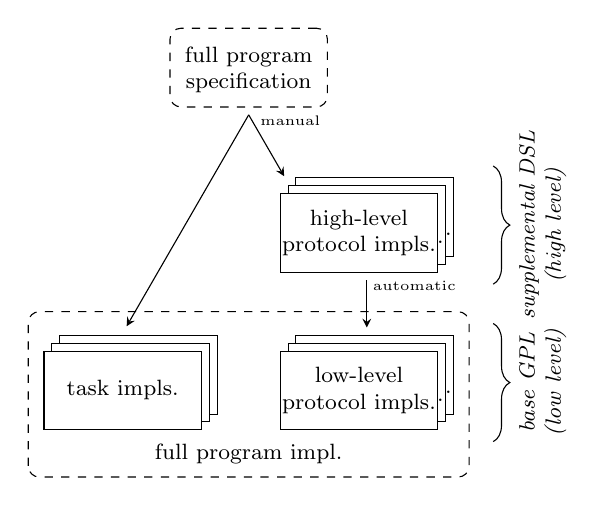
\begin{tikzpicture}[y=-1cm]
		\tikzstyle{box} = [rectangle, draw, minimum width=2cm, minimum height=1cm, inner sep=0pt, align=center, fill=white, outer sep=1mm, font=\footnotesize]
		
		\node [box, dashed, rounded corners] (R) at (0,0) {full program \\ s\smash{p}ecification};
		
		\node [box, xshift=1mm, yshift=1mm] (Pd) at (1.5,2) {high-level \\ protocol impls.};
		\node [box, xshift=0mm, yshift=0mm] (P2) at (1.5,2) {high-level \\ protocol impls.};
		\node [box, xshift=-1mm, yshift=-1mm] (P1) at (1.5,2) {high-level \\ protocol impls.};
		
		\node [box, xshift=1mm, yshift=1mm] (Qd) at (1.5,4) {low-level \\ protocol impls.};
		\node [box, xshift=0mm, yshift=0mm] (Q2) at (1.5,4) {low-level \\ protocol impls.};
		\node [box, xshift=-1mm, yshift=-1mm] (Q1) at (1.5,4) {low-level \\ protocol impls.};
	
		\node [box, xshift=1mm, yshift=1mm] (Td) at (-1.5,4) {task impls.};
		\node [box, xshift=0mm, yshift=0mm] (T2) at (-1.5,4) {task impls.};
		\node [box, xshift=-1mm, yshift=-1mm] (T1) at (-1.5,4) {task impls.};
		
		\draw [-stealth] (R.south) to ($(R.south)+(-60:.9cm)$);
		\draw [-stealth] (R.south) to ($(R.south)+(-120:3.1cm)$);
		\draw [-stealth] ($(P2.south)+(-90:.1cm)$) to ($(P2.south)+(-90:.7cm)$);
		
		\node [anchor=north west, inner sep=0pt, font=\tiny, xshift=4pt] at (R.south) {manual};
		\node [anchor=north west, inner sep=0pt, font=\tiny, xshift=2pt] at ($(P2.south)+(-90:.1cm)$) {automatic};
		
		\draw [dashed, rounded corners] (-2.8,5.2) rectangle (2.8,3.1);
		\node [font=\footnotesize, inner sep=0pt, anchor=south] at (0,5) {\smash{full program impl.}};
		
		
		\draw [decorate, decoration={brace, amplitude=6pt}, xshift=3pt] (3,1.25) to node [rotate=90, anchor=north, yshift=-3pt-1mm, font=\footnotesize\it, align=center] {supplemental DSL \\ (high level)} (3,2.75);
		\draw [decorate, decoration={brace, amplitude=6pt}, xshift=3pt] (3,3.25) to node [rotate=90, anchor=north, yshift=-3pt-1mm, font=\footnotesize\it, align=center] {base GPL \\ (low level)} (3,4.75);
	\end{tikzpicture}
	\caption{Approach}
	\label{fig:approach}
\end{figure}

In recent years, \emph{interaction-centric protocol programming} techniques have
been developed to overcome these and other issues. The idea is that developers
should continue to use an existing GPL (e.g., Java, C, etc.) to implement tasks.
But complementary, developers should use a new domain-specific language (DSL) to
implement protocols. A separate code generator can subsequently translate
high-level protocol implementations in the \emph{supplemental DSL} to low-level
protocol implementations in the \emph{base GPL}; the full program thus emerges
in the base GPL and can be compiled\slash run using its standard tools.
Figure~\ref{fig:approach} illustrates this approach.

A fundamental strength of this approach is that it enforces \emph{modularity} of
protocol code, through the separation of computations and synchronizations\slash
communications. This allows developers to program with procotol-tailored
abstractions, exposed through the DSL; it enables different developers to
implement tasks and protocols separately; it improves ease of reuse and
maintenance; and it better supports reasoning independently about tasks and
protocols. Premier examples of DSLs for protocols are
Reo~\cite{DBLP:journals/mscs/Arbab04} and
Scribble~\cite{DBLP:conf/tgc/YoshidaHNN13}.

\section{Example}

\paragraph{Full program.}

To set the stage for presenting a number of open problems in
Sect.~\ref{sect:open}, imagine we need to implement a Java program with two
tasks, Alice and Bob: Alice repeatedly rolls a die and communicates the outcome
to Bob; Bob repeatedly checks if the outcome equals some value \code{n} (unknown
to Alice); once Alice rolls \code{n}, the program terminates.

\paragraph{Tasks.}

To implement \emph{purely} Alice and Bob, \emph{without the protocol between
them}, concurrency primitives are needed that allow Alice and Bob to indicate
\emph{just} that they are ready to engage in \emph{some} interaction; in turn,
the protocol implementation will decide which \emph{particular} interaction
ensues, beyond Alice's and Bob's control. With Java as our base GPL, we will use
this API that offers such concurrency primitives:

\medbreak
\begingroup
\small
\noindent
\begin{minipage}{.5\linewidth}
\begin{verbatim}
interface Env {
  Object in();
  void out(Object o); }
\end{verbatim}
\end{minipage}
\begin{minipage}{.5\linewidth}
\begin{verbatim}
interface Pr {
  Env env(String name); }

\end{verbatim}
\end{minipage}
\endgroup
\medbreak

\begin{itemize}[leftmargin=.5cm]
	\item \code{Env} -- Represents the \emph{environment} of a task; tasks can use
	methods \code{in}\slash\code{out} to receive\slash send values from\slash to
	their environments, without knowing what exactly their environments consist of.
	Both methods are \emph{blocking}: they complete only once the environment is
	ready.
	
	\code{in}\slash\code{out} have no arguments to indicate the intended
	sender\slash receiver: only \code{Env} objects (i.e., protocol implementations)
	control which values ``flow'' between which tasks.
	
	\item \code{Pr} -- Represents a protocol $P$; it is a container for
	environments, one for every tasks participating in $P$.
\end{itemize}

\noindent We can now implement Alice and Bob as Java methods:

\medbreak
\begingroup
\small
\noindent
\begin{minipage}{.52\linewidth}
\begin{verbatim}
void alice(Env e) {
  Random r = new Random();
  boolean b = false;
  while (!b) {
    e.out(r.nextInt(6));
    b = (boolean)e.in(); } }
\end{verbatim}
\end{minipage}
\begin{minipage}{.48\linewidth}
\begin{verbatim}
void bob(Env e, int n) {
  boolean b = false;
  while (!b) {
    b = (int)e.in() == n;
    out(b); } }

\end{verbatim}
\end{minipage}
\endgroup
\medbreak

\noindent The \code{Env} objects passed to methods \code{alice} and \code{bob}
are instances of \code{Env} classes that are generated from a high-level
protocol implementation in the supplemental DSL. Essentially, the \code{Env}s
ensure \code{alice} and \code{bob} follow the protocol. For instance, the
\code{Env}s ensure that \code{alice}'s first \code{out} blocks until
\code{bob}'s first \code{in} is called (and vice versa); then, they transport
the integer; finally, they unblock \code{alice} and \code{bob}. None of this
logic is in \code{alice} and \code{bob}: it is fully encapsulated in the
\code{Env}s.

The actual integration of the implementations of tasks and protocols is done in
a separate method \code{main}:

\begingroup
\small
\noindent
\begin{verbatim}
void main() {
  Pr p = new AliceBobPr(); // generated
  new Thread(() -> { alice(p.env("A")); }).start();
  new Thread(() -> { bob(p.env("B")); }).start(); }
\end{verbatim}
\endgroup

\paragraph{Protocol.}

\newcommand{\from}{\ \texttt{\small{from}}\ }
\newcommand{\too}{\ \texttt{\small{to}}\ }
\newcommand{\seq}{\texttt{\small;}\ }
\newcommand{\repeatt}{\texttt{\small{repeat}}\ } 

For simplicity, let us use a representative toy supplemental DSL, called
Sequential Binary Communications (SBC); its syntax is inspired by Scribble,
while its formal semantics is inspired by Reo. Let $t$ range over \emph{value
types}, and let $n$ range over \emph{task names}. SBC's grammar looks as
follows:
$$
P \enspace{::=}\enspace t \from n_1 \too n_2 \enspace{\mid}\enspace \repeatt \code{\{}\ P\ \code{\}}
\enspace{\mid}\enspace P_1 \seq P_2
$$
\begin{itemize}[leftmargin=.5cm]
	\item $t \from n_1 \too n_2$ -- synchronous communication of a value typed $t$
	from a task named $n_1$ to a task named $n_2$.
	
	\item
	$\repeatt P$ -- finite number (${\geq}0$) of iterations of $P$.
	
	\item $P_1 \seq P_2$ -- sequential composition of $P_1$ and $P_2$.
\end{itemize}

\noindent
This code implements the protocol between Alice and Bob:

\begingroup
\small
\begin{verbatim}
repeat { int from A to B; boolean from B to A }
\end{verbatim}
\endgroup

\noindent In words, repeatedly, first Alice communicates an integer to Bob, and
then Bob communicates a boolean to Alice.

\newcommand{\comm}{\rightarrowtriangle}

\setlength{\columnsep}{0pt}
\begin{wrapfigure}{r}{3cm}
\centering
\vspace{-.75\baselineskip}
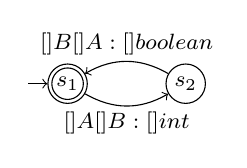
\begin{tikzpicture}
	\tikzstyle{state} = [draw, circle, inner sep=0pt, minimum width=.5cm, x=1.5cm]
	\node [state, font=\footnotesize] (s1) at (0,0) {$s_1$};
	\node [state, font=\footnotesize] (s2) at (1,0) {$s_2$};
	\node [state, minimum width=.4cm] at (0,0) {};
	\draw [->, bend right] (s1) to node [inner sep=2pt, below, font=\footnotesize] {$\code[\footnotesize]{A} \comm \code[\footnotesize]{B} : \code[\footnotesize]{int}$} (s2);
	\draw [->, bend right] (s2) to node [inner sep=2pt, above, font=\footnotesize] {$\code[\footnotesize]{B} \comm \code[\footnotesize]{A} : \code[\footnotesize]{boolean}$}(s1);
	\draw [->] (-.5cm,0) to (s1);
\end{tikzpicture}
\vspace{-\baselineskip}
\end{wrapfigure}
The semantics of SBC can be formalized using \emph{automata} over alphabets of
synchronous communications~\cite{DBLP:journals/scp/JongmansKA17}. For instance,
the automaton for the code above is shown here on the right. This
automaton-based formal semantics is instrumental in three activities:

\begin{itemize}[leftmargin=.5cm]
	\item \emph{Generation of low-level code} -- \code{Env} classes generated for
	an SBC term $P$ essentially simulate $P$'s automaton in an event-driven
	fashion: whenever \code{in}\slash\code{out} is called on an \code{Env} object
	(an event), it checks if this new \code{in}\slash\code{out} \emph{enables} a
	transition out of the current state. If so, the transition is made, and a
	communication ensues; if not, the new \code{in}\slash\code{out} remains pending
	until it can be completed as part of the handling of a next event (cf.
	Reo~\cite{DBLP:conf/tacas/JongmansA16}).
	
	%Automata can also be optimized (e.g., through minimization algorithms) before
	%any low-level code is generated.
	
	\item \emph{Unit testing\slash verification of safety properties} -- A program
	is \emph{(protocol-)safe} iff ``wrong'' \code{in}\slash\code{out} calls never
	complete. To establish safety, one needs to show that \code{Env} objects for a
	protocol never enact interactions that violate some specification. Assuming the
	\code{Env} objects faithfully simulate the protocol's automaton, it suffices to
	show that this automaton meets the protocol's specification. This can be done
	using model-checking (cf. Reo~\cite{DBLP:journals/fac/KokashKV12}).
	
	%As safety can be established purely by analyzing protocol implementations, this
	%is a form of unit testing\slash verification; every protocol implementation is
	%a unit.
	
	\item \emph{Integration testing\slash verification of liveness properties} -- A
	program is \emph{(protocol-)live} iff ``right'' \code{in}\slash\code{out} calls
	always eventually complete. To establish liveness, one needs to show every task
	always eventually calls \code{in}\slash\code{out} in conformance with the
	protocols it participates in (e.g., Alice should first call \code{out} and then
	\code{in}; because, if she first calls \code{out} and then \code{in}, the
	program deadlocks). This can be done by extracting behavioral types from an
	automaton and type-checking tasks against those types (cf.
	Scribble~\cite{DBLP:conf/popl/HondaYC08}).
	
	%As liveness can be established only by analyzing task implementations against
	%protocol implementations, this is a form of integration testing\slash
	%verification.
\end{itemize}

\section{Open Problems}
\label{sect:open}

\begin{enumerate}[leftmargin=.5cm]
	\item How to formally model protocols in a more scalable way? (New automaton
	models? Event structures? Step traces?)
	
	\emph{This is a pivotal open problem: currently, the practical applicability of
	DSLs for protocols is limited by the fact the automata of many realistic
	protocols grow exponentially in the number of tasks. While techniques exist to
	mitigate state explosion, transition explosion is still problematic.}
	
	\item How to optimize the performance of generated code with provably correct
	model transformations, beyond~\cite{jongmans}?
	
	\item How to prove, instead of assume, that \code{Env} objects faithfully
	simulate the automaton for a protocol?
	
	\item How to efficiently \emph{test} safety when protocol models are too large
	to exhaustively \emph{verify}? (Model-based testing?)
	
	\item How to reduce the invasiveness of establishing liveness? (Static code
	analysis without type annotations?)
\end{enumerate}

%%% Acknowledgments
%\begin{acks}                            %% acks environment is optional
%                                        %% contents suppressed with 'anonymous'
%  %% Commands \grantsponsor{<sponsorID>}{<name>}{<url>} and
%  %% \grantnum[<url>]{<sponsorID>}{<number>} should be used to
%  %% acknowledge financial support and will be used by metadata
%  %% extraction tools.
%  This material is based upon work supported by the
%  \grantsponsor{GS100000001}{National Science
%    Foundation}{http://dx.doi.org/10.13039/100000001} under Grant
%  No.~\grantnum{GS100000001}{nnnnnnn} and Grant
%  No.~\grantnum{GS100000001}{mmmmmmm}.  Any opinions, findings, and
%  conclusions or recommendations expressed in this material are those
%  of the author and do not necessarily reflect the views of the
%  National Science Foundation.
%\end{acks}


%% Bibliography
\bibliography{sungshik}


%%% Appendix
%\appendix
%\section{Appendix}
%
%Text of appendix \ldots

\end{document}
